\documentclass[a4paper,english,russian]{G2-105}
\usepackage[T1]{fontenc}
\usepackage{listings}
\usepackage{graphicx}
\usepackage{longtable}
\usepackage{booktabs}
\usepackage{standalone}
\usepackage{newclude}
\usepackage[final]{pdfpages}
\usepackage{multirow}
\usepackage{sansmath} % Enables turning on sans-serif math mode, and using other environments
\sansmath % Enable sans-serif math for rest of document
\usepackage[math]{blindtext}

%\usepackage[utf8]{luainputenc}
\VSTUSetDocumentNumbersPrefix{}
\VSTUSetDocumentCode{ВСТАВИТЬ КОД}
\VSTUSetDocumentTypeDative{выпускной работе бакалавра}
\VSTUSetDocumentTypeGenitive{выпускную работу бакалавра}
\VSTUSetInitialData{задание, выданное научным руководителем с кафедры САПР и ПК,
утвержденное приказом ректора}

\begin{document}
\VSTUSetOrder{????–ст}{??}{??????}{201?}
\VSTUSetFaculty{Электроники и вычислительной техники}
\VSTUSetDepartment{Системы автоматизированного проектирования и ПК}
\VSTUSetDepartmentCode{??.??}
\VSTUSetDirection{??.??.?? Автоматизированные системы управления}
\VSTUSetHeadOfDepartment{Зав. кафедрой САПР и ПК}{д.т.н., ??.}{М. В. Щербаков}{Щербаков Максим Владимирович}
\VSTUSetDirector{старший преподаватель САПР и ПК}{}{А. В. Катаев}{Катаев Александр Вадимович}
\VSTUSetFacilityExpert{}{}{}{}
\VSTUSetStandardsAdviser{????}{?????}{???????????}{?????? ?????? ????????????}
\VSTUSetStudent{ИВТ-461}{Т. А. Мельников}{Мельников Тимофей Алексеевич}
\VSTUSetTitle{Портирование сверточной нейросети на ARM архитектуру с ограниченными вычислительными ресурсами и ресурсами памяти}
\VSTUSetTitleEng{Porting a convolutional neural network on an ARM architecture, taking into account the computing resources and memory resources}
%\VSTUAddChapterWordToTOC % обязательно для ПЗ в магистерских диссертациях
\VSTUInitializePZ
\abstract{Аннотация}
\par Документ представляет собой пояснительную записку к выпускной работе бакалавра на тему «Портирование сверточной нейросети на ARM архитектуру с ограниченными вычислительными ресурсами и ресурсами памяти», выполненную студентом группы ИВТ-461, Мельниковым Тимофеем Алексеевичем.
\par В данной работе рассмотрена возможность реализации алгоритмов машинного обучения, в частности прямой проход сверточной нейронной сети, на устройстве с ограниченными вычислительными ресурсами и ресурсами памяти.
\par Объём пояснительной записки составил \totalpages~страниц и включает \totalfigures~рисунков и \totaltables~таблицы. 

%\newpage
\tableofcontents
\newpage

\starchapter{Введение}
\par Задачи обработки и анализа аналоговой информации являюся одиними из самых сложных в IT-индустрии. Долгое
время такие задачи решались евристическими линейными алгоритмами, которые требовали огромных аппаратных ресурсов при малой точности результата. На протяжении последних десяти лет стремительно растет и развивается прикладная область математики цель которой изучение и развитие искусственных нейронных сетей (НС). Актуальность разработок и исследований в данной области оправдывается применением НС в различных сферах деятельности. Это автоматизация процессов анализа объектов, образов, уневерсализация управления, прогнозирование, создание экспертных систем, анализ неформализованной информации и многие другие применения. В частности, в данной дипломной работе используются нейронные сети для классификации и детектирования объектов на изображении. 
\par Наиболее существенным недостатком НС является их требовательность к вычислительным ресурсам и ресурсам памяти. Частично данная проблема решается использованием сверточных нейронных сетей, которые в виду особенностям логики работы позволяют в разы сократить потребляемые нейронной сетью ресурсы.
\par Не только искусственные нейронные сети являются трендом IT-идустрии, активно развивается коцепция интернета вещей. Диапазон встраиваемых технологий простирается от концепции умных зданий до промышленной консолидации. Интеграция встраиваемых систем и искусственных нейронных сетей позволяет автоматизировать и упростить многие процессы во многих сферах деятельности.
\par В связи с вышесказанным целью данной дипломной работы является внедрение фрейворка машинного обучения на enbedded систему C.H.I.P. и последующая его оптимизация. На основе проделанной работы необходимо сделать вывод о эффективности и рентабельности данного решения. 
\par Для достижения поставленной цели необходимо решить следующие задачи:
\begin{itemize}
\item Изучить фреймворки глубокого машинного обучения
\item Разработать консольное приложение для реализации прямого прохода нейронной сети
\item Оптимизировать использование оперативной памяти и сделать загрузку весов по мере использования
\item Разработать клиент-серверное приложение, демонстрирующее результат работы
\end{itemize}
\par В первом разделе пояснительной записки описаны фрейворки машинного обучения. Далее приведено обоснование выбора фреймворка darknet.
\par Во втором разделе описаны используемые модели нейронных сетей и алгоритм прямого прохода.
\par Третей раздел посвящен разворачиванию фреймворка на устройстве C.H.I.P. и оптимизации работы алгоритма прямого прохода. Так же описана разработка клиент-серверной части для визуализации работы приложения. 
\newpage

\chapter{Обзор фреймворков машинного обучения}
\par Данные раздел содержит справочную информацию, технические особенности и функциональные возможноти фреймворков глубоко машинного обучения и их сравнение. Так же раздел содержит обоснование выбора фреймворка darknet для встраивания и оптимизации на мобильном пк C.H.I.P.
\par Из всего множества фрейворков были выделены Caffe, Torch7, Darknet, как наиболее зрелыe, функционально полныe и широко используемыe.
\section{Caffe}
\par Caffe представляет собой фреймворк, разработанный учеными и практиками, с прозрачной и гибкой архитектурой для глубокого обучения и построения эталонных моделей. Фреймворк распространяется под BSD-лицензией и является c++ библиотекой. Так же реализованы обертки для python и MATLAB для универсализации обучения и развертывания глубоких моделей. Caffe используется на промышленных компаниях и в медиацинтрах, обрабатывая 40 миллионов изображений в день на Titan GPU (примерно 2.5 милисекунд на изображение). Одно из преимуществ Caffe это разделение модели данных от реализации. Что позволяет использовать приложения на разных платформах.
\par Caffe поддерживается и разрабатывается университетом Беркли, а именно центром BVLC.
\subsection{Основыне характеристики Caffe}
\par Caffe представляет полный набор инструментов для обучения, тестирования, настройки и разработки можелей с подробной документацией и разобранными примерами. Поэтому процесс обучение использования фреймворка занимает короткий период. Возможность использования GPU делает Caffe одним из самых быстрых фреймворков, что позволяет его использовать в промышленном секторе. Такие показатели достигнуты благодаря особенностям описаным ниже.
\par Caffe является модульным программным обеспечением. Что позволяет легко добалять новые форматы данных, слои и функции потерь. В фреймворке уже реализовано множество слоев и функций потерь, что позволяет реалзовавать нейронную сеть для задачь различных предметных областей и категорий.
\par В Caffe представление и реализация разделены. Для описания модели в Caffe используется конфигурационный файл в формате protobuf. Caffe поддерживает сетевые архитектуры в форме произвольно ориентированных ациклических графов. Важным деталей является то, что после создания экземпляра модели Caffe выделяется ровно столько памяти, сколько необходимо для работы сериализованной нейронной сети и для хранения адреса объекта.[1]
\par В Caffe используется полное тестовое покрытие. Каждый модуль имеет собственный набор тестов. Модуль будет принят, только после прохождение всего набора тестов. Это позволяет эффективно оптимизировать модули и гарантирует стабильную работу фреймворка.
\par Caffe содержит предворительно обученные модели для академических целей и некоммерческого использования. Доступны сверточные НС с архитектурой "AlexNet" и вариации данной НС, обученные на базе данных ImageNet[2]. Так же доступны реккурентные модели[3].
\subsection{Приемущества Caffe}
\par От других современных фреймворков глубокого обучения Caffe отличается следующими качествами(!):
\begin{itemize}
	\item Реализция полностью основана на C++, что облегчает интеграцию с встраиваемыми системами. CPU режим позволяет использовать фреймворк без специализированного GPU.
	\item Готовые модели позволяют не тратитб время и ресурсы на обучение. Важным пунктом является подробная документация для сериализации и использовании моделей.
\end{itemize}
\subsection{Архитектура Caffe}
\par Caffe сохраняет и передает данные в четырехмерных массивах, которые названы блобами. Блобы представляют унифицированный интерфейс для работы  памятью, содержащий пакеты ихображений (или других данных), параметров или обновлений параметров. Блобы скрывают вычислительные издержки смешанной работы CPU и GPU, выполняя синхронихацию по нере необходимости. Память выделяется по требованию (лениво), что позволяет эффективней ее использовать. Модели сохраняются как буфер, использующий протокол Google (Google Protocol Buffers), который имеет ряд достоинст: минимальный размер строки при сериализации, эфективная сериализация, высокая читабельность в текстовом виде и удобные интерфейсы работы на нескольких языках. Необходимые для обучения огромные массивы данных храняться в базах данныx LevelDB. Google Protocol Buffers и LevelDB обеспечивают пропускную способность в 150 Мб/с. 
\par Слой в Caffe представляет собой структуру соответствующую формальному определению слоя: он принимает на вход один или несколько блобов и выдает один или несколько блобов результатом. Caffe предоставляет полный набор типов слоев для глубокого обучения, включая сверточный, pooling слой, inner products слой, нелиности, такие как выпремленная линейная и логическая, слои потерь, таких как softmax и hinge. Настройка слой требует минимальных усилий в виду композиционного построения сетей.
\par Caffe обеспечивает функциональность для любого направценного ациклического графа слоев, позволяя корректно выполнять прямой и обратный проход. Модели Caffe --- это сквозные системы машинного обучения.[1]

\section{Torch7}
\par Torch7 --- это универсальный математический фреймворк и библиотека машинного обучения, которая имеет оболочку для языка программирования Lua. Его цель --- предоставить гибкую среду для проектирования и обучения моделей глубокого обучения. Гибкость достигается с помощью Lua, так как он является очень легким скриптовым языком. Эффективная реализация низкоуровневых числовых процедур, используя OpenMP и CUDA, позволяет фрейморку достич выской производительности. Фреймворк имеет простой Lua-интерфейс, что позволяет легко подключать его к стороннему программному обеспечению.
\subsection{Основыне характеристики Torch7}
\par Структура фрейворка имеет три основных преимущества:
\begin{itemize}
\item она облегчает разработку численных методов;
\item фреймворк легко расширяем (включая использование сторонних библиотек);
\item высокая скорость работы фреймворка.
\end{itemize}
\par Второе преимущества достигается за счет выбранных разработчиками технологий. Скрипровый (интерпретируемый) язык с хорошим API-интерфейсом для C обеспечивает фреймворку гибкост в разработке и не накладывает ограничения на   его расширяемость. Так как, язык высокого уровня делает процесс разработки программы более простым и понятным, чем язык низкого уровня. К тому же, интерпретируемость позволяет быстро и легко реализовывать различные идеи в интерактивном режиме. Хороший API-интерфейс сохраняет функциональные возможности из разных библиотек, так как становиться прослойкой между универсальной структурой на языке Lua и различными структурами используемых библиотек на языке C.
\par Высокая скорость работы достигается благодаря компилятору JIT (Just In Time). На данный момет Lua является самым быстрым интерпритируемым языком. Lua разрабатывался для легкого внедрения в приложения, написанные на C. Поэтому представляет большое C-API на основе виртуального стека, для передачи значений между Lua и C. Это унифицирует интерфейс для C/C++ и делает обертывание библиотек тривиальным. [4]
\par Lua предназначен для использования в качестве мощного, легкого скриптового языка обладающими всеми необходимыми выразительными средствами. Он реализован как библиотека, которая написана на чистом C (точнее на подмножестве ANSI C и C++). Lua сочетает простой процедурный синтаксис с мощными конструкциями описания данных на основе ассоциативных массивов и расширяемой семантики. Lua динамически типизируется, выполняется путем интерпретации байт-кода для виртуальной машины на основе регистров и имеет автоматическое управление памятью с инкрементной сборкой мусора, что делает его идеальным для настройки, написания сценариев и быстрого прототипирования.[5]
\par Lua предлагает хорошую поддержку объектно-ориентированного программирования, функционального программирования и программирования, управляемого данными. Основным типом Lua является таблица, которая реализует ассоциативные массивы очень эффективным способом. Ассоциативный массив --- это массив, который может индексироваться не только числами, но и любыми другими типами данных язка. Таблицы не имеют фиксированного размера, они динамически изменяемы и могут использоваться как "виртуальные таблицы" над другой таблицей, что позволяет имитировать парадигмы объектно-ориентированного программирования. Таблицы являются единственным, но очень мощным механизмом структурирования данных в Lua. Torch7 использует таблицы для простого, равномерного и эффективного представления обычных массивов, таблиц символов, кортежей, очередей и других структур данных. Lua также использует таблицы для представления пакетов.
\par Lua и Python очень схожи как по структурированию данных, так и по стилю программирования. Если говорить о популярности в сообществе, то Python опережает Lua из-за огромного количества поставляемых библиотек. Однако разработчики выбрали Lua по ряду других причин, которые, в виду специфики фреймворка, являются ключевыми. Во-первых, интеграция Lua с C очень проста. За несколько часов любая библиотека на C или C++ может стать библиотекой Lua. Во-вторых, Lua предоставляет эффективные возможности встраивания. Что бы преобразовать прототип в финальный продукт требуется не много дополнительной работы. В-третьих, Lua обладает высокой производительностью благорадя интерпритатору LuaJIT, который дает производительность на уровне C. Еще одним преимуществом Lua является переносимость. Lua написан на чистом ANSI C, его можно скомпилировать для любых устройств (сотовые телефоны, встроенные процессоры в FPGA, процессоры DSP и др.).
\subsection{Структуры используемых данных}
\par Ключевой сущностью в Torch7 является класс Tensor, поставляемый автономной С-библиотекой Tensor. Данный класс расширяет базовый набор типов Lua, чтобы реализовать эффективную работу с многомерными массивами. Большинство пакетов Torch7 или сторонних пакетов, зависящих от Torch7, реализуют собственный класс Tensor для представления сигналов, изображений, видео и других объектов, что делает интегрирование различных библиотек тривиальной задачей. Библиотека Torch Tensor предоставляет множество классическ их операций (включая операции линецной алгебры), который реализованны и оптимизированны на С, используются SSE интсрукции для Intel платформ. Опцианально можно использовать высокопроизовидельные реализации BLAS/Lapack операций линейной алгебры. Так же данная библиотека поддерживает инструкции OpenMP и вычисления на CUDA GPU.
\subsection{Пакеты Torch7}
\par На данный момент Torch7 имеет 8 встроенных пакетов:
\begin{itemize}
\item torch: основной пакет Torch7. Обеспечивает фреймворк классом Tensor, облегчает сереализацию и другие базовые функции;
\item lap и plot: представляют стандартные функции для создания, преобрзования и визуализации объектов Tensor. Пример работы показан на рисунке ~\ref{torch_plots}
\begin{figure}
    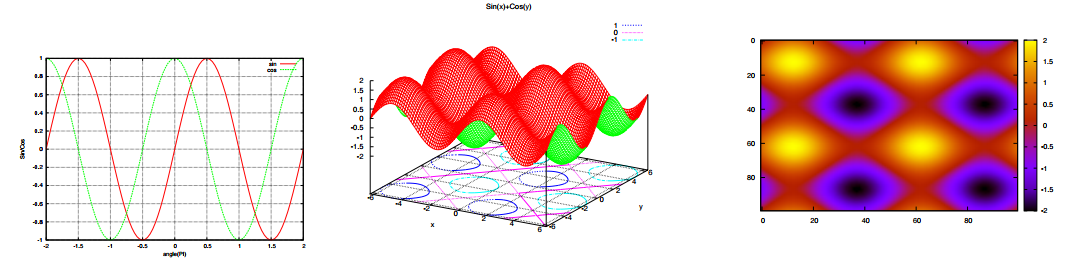
\includegraphics[width=\linewidth]{torch_plots.png}
    \caption{Графики, полученные с помощую пакета plot фреймворка Torch7. Слева: простые синусоидальные функций. В центре: Поверхность, хранящаяся в 2D Tensor. Справа: Матричный график, построенный с использованием карты тепла}
	\label{torch_plots}
\end{figure}
\item qt: предаставляет интерфейс работы Torch7 с Qt. Реализует конфертацию Tensor в QImage и наоборот. Отлично подходит для быстрого создания интерактивных демонстраци с кроссплатформенным графическим интерфейсом.
\item nn: предоставляет набод стандартных модулей для создания нейронной сети. В пакет так же входит набор контейнерных модулей, которые можно использовать для определения произвольно направленных графов. Явное описание графа позволяет избежать сложности с анализатором графов или любого другого компилятора промежуточного уровня.
\par На практике нейронная сеть представляет собой последовательные графы, либо имеют шаблонные витвления и рекурсии. На рисунке ~\ref{nn_create} показано создание многослойного перцептрона.
\begin{figure}
    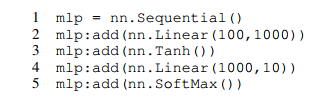
\includegraphics[width=0.3\paperheight]{nn_create.png}
    \caption{Создание многослойного перцептрона, используя пакет nn}
	\label{nn_create}
\end{figure}
\end{itemize}


\chapter{Используемые алгоритмы и модели}
\section{Теоретические основы нейронных сетей}
\subsection{Перцептрон - основа нейронных сетей}
\par В основе современной концепции 

\chapter{Проектирование системы}


\newpage
\starchapter{Заключение}
\newpage
\begin{thebibliography}{1}
    \bibitem{1} https://arxiv.org/pdf/1408.5093.pdf
    \bibitem{2} J. Donahue, Y. Jia, O. Vinyals, J. Hoffman, N. Zhang, 
E. Tzeng, and T. Darrell. Decaf: A deep convolutional
activation feature for generic visual recognition. In ICML,
2014
  	\bibitem{3}  A. Krizhevsky, I. Sutskever, and G. Hinton. ImageNet
classification with deep convolutional neural networks. In
NIPS, 2012
	\bibitem{4} http://ronan.collobert.com/pub/matos/2011\_torch7\_nipsw.pdf
	\bibitem{5} http://www.lua.ru/doc/1.html
\end{thebibliography}


\appendixdocument{Техническое задание}
\end{document}